\documentclass[conference,12pt,onecolumn,draftclsnofoot,a4paper]{IEEEtran}

\usepackage[final]{pdfpages}

\usepackage{float}
\usepackage{tabularx}
\usepackage{hyperref}
\usepackage{amssymb}
\usepackage{subcaption}

\usepackage{fancyhdr} 
\fancyhf{}
\renewcommand{\headrulewidth}{0pt}
\renewcommand{\footrulewidth}{0pt}
\cfoot{\thepage}
\pagestyle{fancy} 


\title{Basic IEEE Style Document}
\author{\IEEEauthorblockN{Dean Mills}
\IEEEauthorblockA{University of Pretoria\\
Email: u13081650@tuks.co.za}}

\begin{document}

\title{Depth-Infused Graph Attention Networks for Real-Time Multi-Person Pose Tracking}
\author{Dean Mills}

\input{declaration_of_originality}

\maketitle

\begin{abstract} 
This proposal outlines a detector-agnostic framework for
multi-person pose tracking in single images. A monocular depth estimator first
augments each detected keypoint with a depth value, lifting the 2-D skeleton
into 2.5-D space. The enriched joints are represented as nodes in a graph whose
edges encode spatial and geometric relationships; a depth-aware Graph Attention
Network (GAT) then learns attention weights that group joints into coherent
person-specific skeletons. The framework accepts input from any off-the-shelf
pose detector—convolutional or transformer-based—and aims to improve
joint-to-person assignment accuracy in crowded scenes while preserving
real-time performance and reducing training time through a more compact,
graph-based feature space. 
\end{abstract}

\begin{IEEEkeywords}
    Pose Estimation, Pose Tracking, Multi-Person Pose Tracking, Graph Attention Networks, Vision Transformers, Monocular Depth
\end{IEEEkeywords}

\section{Introduction}
Human pose estimation refers to the task of locating the principal body
joints—such as elbows, knees, and shoulders—within an image. The exact list of
joints depends on the data set: \textsc{COCO-WholeBody} annotates seventeen
body keypoints in addition to detailed hand, foot, and face landmarks
\cite{jin2020whole}, whereas the Leeds Sports Pose data set provides fourteen
body keypoints \cite{johnson2010clustered}. Over the past decade the field has
converged on two broad pipelines. In a \emph{top-down} pipeline, each person is
first enclosed in a bounding box and the keypoints are predicted inside that
region; in a \emph{bottom-up} pipeline, every visible joint is detected in a
single pass and a grouping stage later assembles them into individual
skeletons. Before the deep-learning era, solutions combined handcrafted image
descriptors with relatively shallow learners. Examples include relevance-vector
machines \cite{tipping2001sparse}, mixtures of experts
\cite{sigal2006predicting}, locality-constrained coding
\cite{wang2010locality}, relevant-component analysis \cite{kanaujia2007semi},
bag-of-words representations \cite{ning2008discriminative}, random forests
\cite{chang2013fast}, Hough forests \cite{girshick2011efficient}, pixel- and
superpixel-level models \cite{wang2011multi}, and motion cues
\cite{sapp2013modec}. While these methods laid the essential groundwork,
limited representational capacity hampered their performance and they naturally
struggled to compete with more modern approaches.

Deep convolutional networks (CNNs) \cite{lecun1998gradient} transformed the
task by learning features directly from data. \textsc{DeepPose} (revolutionary
at the time) \cite{toshev2014deeppose}, based on the eight-layer AlexNet
backbone \cite{krizhevsky2012imagenet}, was the first model to show that an
end-to-end CNN could localise human joints reliably. Subsequent architectures
escalated both depth and representational capacity: VGGnet with 16-19 layers
\cite{simonyan2014very}; ResNet with 50, 101, or 152 layers linked by residual
shortcuts \cite{he2016deep}; and, later, High-Resolution Networks (HRNet) that
maintain parallel feature streams at multiple resolutions throughout the
network \cite{sun2019deep}. On top of these backbones, researchers introduced
multi-stage refinement modules that progressively sharpen coarse heat-maps into
precise keypoint locations—examples include Convolutional Pose Machines
\cite{wei2016convolutional}, stacked hourglass networks
\cite{newell2016stacked}, and the part-affinity field branch used by
\textsc{OpenPose} \cite{cao2017realtime}. Additional variants (all using some
convolution backbone), such as Cascade Feature Aggregation
\cite{su2019cascade}, SimpleBaseline \cite{xiao2018simple}, and the Cascaded
Pyramid Network \cite{chen2018cascaded}, improved accuracy, but each gain was
accompanied by additional layers, parameters, and computational cost (this is a
relatively broad statement but it does describe the trend).

More recently, vision transformers have emerged as a versatile alternative to
convolutional backbones, replacing local convolution with multi-head
self-attention so that every image patch -- or any intermediate "token" standing
in for a joint -- can exchange information with all others in a single layer
\cite{vaswani2017attention}. In practice the image (or a coarse set of
heat-maps) is converted into a token sequence, processed by stacked transformer
blocks that model long-range dependencies, and then decoded back into keypoint
coordinates. Variations on this theme include \textsc{TokenPose}, which
attaches a learnable token to each joint and passes the sequence through a
transformer encoder \cite{li2021tokenpose}; \textsc{HRFormer}, which retains
HRNet's multi-resolution branches but fuses them with windowed attention
\cite{yuan2021hrformer}; and \textsc{ViTPose}, which drops the convolutional
stem entirely and shows that a plain Vision Transformer can match or surpass
CNN baselines when enough data are available \cite{xu2022vitpose}. Transformer
backbones are offered in graded sizes -- small models that run in real time on
consumer GPUs, medium models that balance speed and accuracy, and large models
whose parameter counts approach a billion or more -- so speed/accuracy trade-offs
can be made by selecting a lighter or heavier version of the \emph{same
architecture} rather than rebuilding the entire network.

Depth cues provide a complementary signal that helps disambiguate overlapping
limbs. Monocular predictors such as \textsc{MiDaS}, trained on a broad
collection of real-world data sets \cite{ranftl2021robust,ranftl2022dense}, and
\textsc{ZoeDepth}, which mixes real and synthetic images to widen scene
coverage \cite{khattak2023zoedepth}, now produce accurate, scale-consistent
depth maps with a single forward pass. Attaching the estimated depth value to
each keypoint effectively lifts the 2-D skeleton into 2.5-D space, offering
geometric context that pure image coordinates lack.

Multi-person scenes remain challenging because joints belonging to different
individuals often overlap or lie in close proximity, making \emph{pose
tracking} -- the task of grouping detected joints into the correct person-specific
skeletons -- non-trivial. One approach is to represent the estimated skeleton as a
graph in which each node corresponds to a joint and each edge encodes spatial
or geometric relationships between joints; a Graph Attention Network (GAT) then
learns attention weights that highlight the most informative neighbours
\cite{velivckovic2017graph}. This paper proposes a \emph{depth-aware} GAT that
combines 2-D image coordinates with per-joint depth values, remains
detector-agnostic -- able to consume keypoints from either a lightweight ResNet
heat-map head or a transformer front-end (as examples) -- and is designed to
improve the accuracy and real-time performance of pose tracking in crowded
scenes.
\section{Background}

This section reviews the key concepts underlying the proposed method -- graphs,
graph-based neural networks, and monocular depth estimation for lifting 2-D
joint coordinates to 2.5-D.

\subsection{Graphs}
Graphs are a versatile structure for representing complex relationships between
entities. A graph consists of nodes (or vertices) and edges (or links) that
connect pairs of nodes, making it particularly suitable for modeling data where
relationships are central, such as the connections between human joints in pose
estimation.

In formal terms, a graph \( G = (V, E) \) includes:
\begin{itemize}
  \item A set of nodes \( V \), representing the entities.
  \item A set of edges \( E \), where each edge \( e \in E \) connects two nodes
  \( (u, v) \), with \( u, v \in V \).
\end{itemize}

Graphs may be directed or undirected, depending on whether the connections
between nodes have a specific direction. This flexibility enables graphs to
effectively capture the various types of relationships that may be beneficial 
for pose estimation.

\subsection{Graph Neural Networks}
Graph Neural Networks (GNNs) \cite{scarselli2008graph} are a class of neural
networks designed to operate on graph-structured data. Unlike traditional neural
networks that work on structured data, GNNs are tailored to handle the irregular
structure of graphs. The fundamental idea behind GNNs is the message passing
framework, which allows nodes to iteratively exchange information with their
neighbors to update their own representations.

In the message passing framework, each node is initially assigned a feature
vector. During each iteration, a node aggregates messages from its neighboring
nodes. This process can be summarized in two main steps:
\begin{itemize}
  \item \textbf{Message Aggregation}: At each iteration \( t \), a node \( v \)
  collects messages from its neighboring nodes \( \mathcal{N}(v) \):
  \begin{equation}
    m_v^{(t+1)} = \mathrm{AGGREGATE}^{(t)} \left( \{ h_u^{(t)} : u \in \mathcal{N}(v) \} \right)
  \end{equation}
  Here, the aggregation function could be a sum, mean, or max function, which
  combines the features of neighboring nodes.
  \item \textbf{Node Update}: After aggregation, the node updates its feature
  vector based on the collected messages:
  \begin{equation}
    h_v^{(t+1)} = \mathrm{UPDATE}^{(t)}(h_v^{(t)}, m_v^{(t+1)})
  \end{equation}
  The update function often involves applying a non-linear transformation, such
  as a neural network layer, to the aggregated messages and the node's current
  state.
\end{itemize}
This iterative process allows each node to refine its representation by
incorporating information from its neighbors, effectively capturing the
dependencies within the graph.

\subsection{Graph Convolutional Networks}
Graph Convolutional Networks (GCNs) \cite{kipf2016semi} are a specialized type
of GNN that extend the idea of convolution from grid-like data structures to
graphs. In a GCN, the convolution operation is adapted to aggregate information
from a node's local neighborhood, enabling the network to learn features that
are informed by the local context within the graph.

A typical GCN layer is defined as:
  \begin{equation}
    H^{(t+1)} = \sigma \left( \tilde{D}^{-1/2} \tilde{A} \tilde{D}^{-1/2} H^{(t)} W^{(t)} \right)
  \end{equation}
where:
\begin{itemize}
  \item \( \tilde{A} = A + I \) is the adjacency matrix of the graph, with added
  self-loops to include the node's own features in the aggregation.
  \item \( \tilde{D} \) is the degree matrix corresponding to \( \tilde{A} \),
  used for normalization.
  \item \( H^{(t)} \) represents the feature matrix at layer \( t \), where each
  row corresponds to a node's features.
  \item \( W^{(t)} \) is the trainable weight matrix for the layer.
  \item \( \sigma \) denotes an activation function, such as ReLU, applied
  element-wise to introduce non-linearity.
\end{itemize}
This layer allows the network to capture the structural information of a node's
neighborhood, leading to more contextually informed node representations.

\subsection{Graph Attention Networks}
Graph Attention Networks (GATs) \cite{velivckovic2017graph} introduce an
attention mechanism (this mechanism is notably used in transformers
\cite{vaswani2017attention} which are the backbone of large language models
\cite{zhao2023survey}) into the GNN framework, allowing the network to assign
different levels of importance to different neighbors during the aggregation
process. This is particularly useful in scenarios where certain neighbors
contribute more significantly to a node's representation than others.

The key steps in a GAT layer are:
\begin{itemize}
  \item \textbf{Self-Attention Mechanism}: For each pair of connected nodes \(
  (u, v) \), an attention coefficient is computed to measure the importance of
  node \( u \)’s features to node \( v \):
  \begin{equation}
    e_{uv} = \mathrm{LeakyReLU} \left( \mathbf{a}^T \left[ W h_u \, || \, W h_v \right] \right)
  \end{equation}
  Here, \( \mathbf{a} \) is a learnable weight vector, \( W \) is a shared
  weight matrix, and \( || \) denotes concatenation.
  \item \textbf{Normalization}: The attention coefficients are normalized across
  all neighbors of a node using the softmax function:
  \begin{equation}
    \alpha_{uv} = \frac{\exp(e_{uv})}{\sum_{k \in \mathcal{N}(v)} \exp(e_{vk})}
  \end{equation}
  This normalization ensures that the sum of the attention weights for each node
  is 1.
  \item \textbf{Aggregation}: Each node’s new feature is computed as a weighted
  sum of its neighbors’ features, with the attention coefficients serving as
  weights:
  \begin{equation}
    h_v' = \sigma \left( \sum_{u \in \mathcal{N}(v)} \alpha_{uv} W h_u \right)
  \end{equation}
  The result is a more nuanced node representation that accounts for the varying
  significance of different neighbors, improving the network's ability to learn
  complex patterns in the data.
\end{itemize}

\subsection{Monocular Depth Estimation} 

Monocular depth estimation infers a dense depth map $D \in \mathbb{R}^{H \times
W}$ from a single RGB image $I \in \mathbb{R}^{H \times W \times 3}$. Because
absolute scale is ambiguous in a single view, networks learn scene priors that
connect image appearance to plausible metric or relative depth. Most
contemporary methods follow an encoder–decoder pattern first popularised by
multi-scale CNNs \cite{eigen2014depth,laina2016deeper}: an encoder extracts
hierarchical features, and a decoder progressively upsamples them—often with
skip connections or multi-scale refinement—to yield per-pixel depth
predictions.

Training regimes fall into two broad categories. \emph{Supervised} approaches
optimise losses such as $\ell_1$, $\ell_2$, or scale-invariant errors against
ground-truth depth captured with active sensors or multiview reconstruction
\cite{laina2016deeper}. \emph{Self-supervised} approaches eliminate depth
labels altogether and instead enforce photometric consistency across stereo
pairs or successive video frames, using differentiable view synthesis and
occlusion masks \cite{godard2017unsupervised,zhou2017unsupervised}.

Recent sota models illustrate the maturation of the field. \textsc{MiDaS}
combines a vision-transformer encoder with a multi-resolution decoder and is
trained on a heterogeneous mixture of data sets to generalise across domains
\cite{ranftl2021robust,ranftl2022dense}. \textsc{ZoeDepth} extends this idea by
mixing real and synthetically rendered images \cite{khattak2023zoedepth}. These
networks now deliver accurate, scale-consistent depth maps with a single
forward pass, making depth a reliable signal for vision tasks.
\section{Research Objectives}

The overarching goal of this study is to design and analyse a detector-agnostic
framework for multi-person pose tracking that couples a depth-aware graph
representation with a Graph Attention Network (GAT).  
Within this broad aim, the work pursues four concrete objectives:

\begin{itemize}
    \item \textbf{Depth-Aware Graph Construction}\,:  
    Formulate a graph in which each node stores a joint’s image coordinates and
    estimated depth while each edge encodes spatial and geometric relations;
    analyse how the added depth channel alters feature compactness and
    expressiveness compared with purely 2-D graphs.

    \item \textbf{Accurate Joint-to-Person Assignment}\,:  
    Investigate whether incorporating depth into the GAT improves joint
    grouping accuracy in crowded scenes where limbs from different individuals
    overlap or appear in close proximity.

    \item \textbf{Computational Efficiency}\,:  
    Evaluate whether the compact, graph-based feature space shortens training
    time and sustains real-time inference, identifying trade-offs between model
    depth, runtime, and memory footprint.

    \item \textbf{Detector-Agnostic Scalability}\,:  
    Demonstrate that the framework can ingest keypoints produced by diverse
    detectors—ranging from lightweight CNN heads to transformer
    architectures—without architectural changes, and analyse performance
    sensitivity to the underlying detector.
\end{itemize}

Together, these objectives target a pose-tracking solution that is accurate in
crowded settings, computationally practical, and readily transferable across 
pose detection front-ends.
\section{Datasets}

Progress in human pose estimation and tracking has been driven by a variety of
data sets that differ in scale, keypoint layout, media type (static images
versus video sequences), and scene complexity. The MPII Human Pose data set
provides roughly 25\,000 images with sixteen annotated joints collected from
everyday activities \cite{andriluka14cvpr}, whereas MS~COCO supplies more than
200\,000 images and 250\,000 person instances labelled with seventeen
keypoints, covering a wide range of body sizes, viewpoints, and occlusion
patterns \cite{lin2014microsoft}.

For the present study the primary requirement is a large, widely adopted data
set that follows the standard seventeen-joint schema and includes multi-person
annotations; MS~COCO satisfies these criteria and therefore serves as the main
benchmark. Additional data sets listed in Table~\ref{tab:datasets} remain
valuable for several reasons: CrowdPose \cite{li2019crowdpose} and PoseTrack
\cite{andriluka2018posetrack} feature dense crowds; COCO-WholeBody
\cite{jin2020whole} and Halpe \cite{alphapose} extend the annotation to hands,
feet, and facial landmarks, enabling experiments on fine-grained keypoints; and
video-based sets such as JTA \cite{fabbri2018learning} and 3DPW
\cite{vonMarcard2018} offer temporal information for sequence tracking.

\begin{table}[H] \centering \begin{tabular}{|l|c|c|c|} \hline \textbf{Dataset}
& \textbf{Images/Sequences} & \textbf{\# Keypoints} & \textbf{Multi-person} \\
\hline MPII \cite{andriluka14cvpr} & 25K & 16 & \checkmark \\ \hline MPII-TRB
\cite{duan2019trb} & 25K & 40 & \checkmark \\ \hline CrowdPose
\cite{li2019crowdpose} & 20K & 14 & \checkmark \\ \hline PoseTrack
\cite{andriluka2018posetrack} & 23K & 15 & \checkmark \\ \hline AI Challenger
\cite{wu2017ai} & 300K & 14 & \checkmark \\ \hline COCO \cite{lin2014microsoft}
& 200K & 17 & \checkmark \\ \hline Halpe \cite{alphapose} & 43K & 136 &
\checkmark \\ \hline COCO-WholeBody \cite{jin2020whole} & 200K & 133 (17 body)
& \checkmark \\ \hline FLIC \cite{sapp2013modec} & 5K & 10 & \\ \hline LSP
\cite{johnson2010clustered} & 2K & 14 & \\ \hline Human3.6M
\cite{ionescu2013human3} & 3.6M & 32 & \\ \hline
%https://github.com/chaneyddtt/Generating-Multiple-Hypotheses-for-3D-Human-Pose-Estimation-with-Mixture-Density-Network/issues/12
MPI-INF-3DHP \cite{mehta2017monocular} & 1.3M & 29 & \\ \hline SURREAL
\cite{varol17_surreal} & 6M & 24 & \\ \hline JTA \cite{fabbri2018learning} &
512 videos & 21 & \checkmark \\ \hline 3DPW \cite{vonMarcard2018} & 60
sequences & 17 & \checkmark \\ \hline MARCOnI \cite{EEJTP15} & 12 sequences &
25 & \checkmark (not all sequences) \\ \hline TUM Kitchen \cite{tenorth2009tum}
& 20 sequences & 28 & \\ \hline \end{tabular} \caption{Summary of key human
pose estimation datasets.} \label{tab:datasets} \end{table}
\section{Metrics Used in Pose Estimation and Tracking}
Evaluating the performance of pose estimation and tracking models involves a
variety of metrics, each designed to measure the accuracy and effectiveness of
predicted joint positions and overall tracking performance. These metrics
revolve around the accuracy of the predicted points compared to the ground
truth, assessing how well the model identifies and tracks keypoints across
images or video sequences.

\subsection{Pose Estimation Metrics}
Pose estimation metrics primarily focus on the accuracy of detecting individual
body joints. Below are some of the key metrics used in the evaluation of pose
estimation:

\textbf{Percentage of Correct Parts (PCP)} \cite{kiefel2014human}: Initially a
standard in the field, PCP measures the accuracy of limb detection. A limb is
considered correctly detected if the distance between the predicted and actual
joint positions is less than half the limb's length. However, PCP has been
criticized for its bias against shorter limbs, leading to its decline in
popularity.

\textbf{Percentage of Detected Joints (PDJ)} \cite{abobakr2016body}: PDJ was
developed to address the limitations of PCP. It measures the accuracy of joint
detection based on the proximity of the predicted joint to its true position,
relative to the torso's diameter. This metric allows for different levels of
localization precision by adjusting the acceptable error threshold.

\textbf{Percentage of Correct Keypoints (PCK)} \cite{gouidis2019accurate}:
Similar to PDJ, PCK evaluates the proximity of predicted joint locations to
their true counterparts but uses the maximum dimension of the ground truth
bounding box as the reference. This metric provides a measure of localization
accuracy for body joints.

\textbf{PCKh} \cite{andriluka20142d}: An adaptation of PCK, PCKh uses the head
segment length to normalize the matching threshold, accounting for individual
size differences. The threshold is set at 50\% of the head segment length,
promoting a size-independent evaluation of joint detection accuracy.

\textbf{Area Under the Curve (AUC)} \cite{guler2018densepose}: This metric
reviews the model's performance across varying PCK thresholds, illustrating its
capability to accurately localize body joints over a range of precision levels.

\textbf{Object Keypoint Similarity (OKS) \cite{maji2022yolo}}: Analogous to
Intersection over Union (IoU) \cite{rezatofighi2019generalized} in object
detection, OKS assesses how closely the predicted keypoints match the actual
data points, emphasizing the quality of overlap between predicted and true
keypoints.

\subsection{Pose Tracking Metrics}
For multi-person pose tracking, additional metrics are used to evaluate the
accuracy of tracking across frames in a video sequence. These metrics are
derived from Multiple Object Tracking (MOT) metrics \cite{milan2016mot16} and
focus on how well the model maintains the identity and position of detected
joints over time:

\textbf{Multiple Object Tracking Accuracy (MOTA)}
\cite{bernardin2008evaluating}: MOTA is a metric used to evaluate the overall
performance of a tracking system. It takes into account three key factors: false
positives (when the system incorrectly identifies a non-existent object), false
negatives (when the system fails to detect an actual object), and identity
switches (when the system mistakenly assigns a different identity to an already
tracked object). By considering these factors, MOTA provides a comprehensive
assessment of the system's accuracy. It calculates this accuracy by averaging
the tracking performance for each joint across all body joints, making it an
important measure of how effectively the model tracks multiple people over time.

\textbf{Multiple Object Tracking Precision (MOTP)}
\cite{bernardin2008evaluating}: MOTP measures the precision of the predicted
joint positions relative to the ground truth, focusing on how accurately the
model tracks the position of each joint. High MOTP values indicate that the
predicted joint locations are close to their true positions.

\textbf{Precision and Recall}: These metrics evaluate the proportion of
correctly identified joints (Precision) and the proportion of true joints
correctly detected (Recall) (The Average Precision and Average Recall metrics
used in \cite{Chen_2018_CVPR}). High precision and recall indicate that the
model is effective at detecting and tracking body joints without missing or
incorrectly identifying them.

\textbf{Mean Average Precision (mAP)}: Mean Average Precision (mAP) is employed
to assess frame-wise multi-person pose accuracy, as described in
\cite{pishchulin2016deepcut}. The mAP metric evaluates how accurately each
person is detected and localized within a frame, accounting for both detection
and localization errors. Traditionally, mAP evaluation depends on knowing the
location and rough scale of a group of individuals during evaluation. However,
in realistic scenarios, particularly in video contexts, such ground-truth
information is rarely available.

These metrics collectively provide a comprehensive framework for evaluating the
performance of multi-person pose tracking models. By combining measures of
accuracy, precision, and recall with the mAP metric, these evaluations offer
insights into both the localization and tracking capabilities of the models
across complex and dynamic video sequences.

\subsection{Challenges in Multi-Person Pose Tracking}
The evaluation of multi-person pose tracking models reveals that tracking
accuracy significantly decreases with the increased complexity of video
sequences/images. Simple data with clearly separated individuals in upright poses
generally result in high tracking accuracy, while data involving
overlapping individuals, fast movements, and complex body articulations tend to
challenge the tracking algorithms, leading to lower MOTA scores. The
relationship between pose estimation accuracy and tracking performance often
shows that better pose estimation corresponds to better tracking, though there
are exceptions where accurate pose estimation does not translate to effective
tracking due to the challenges posed by complex scenes.
\section{Hypothesis}

This research hypothesises that representing detected joints as nodes in a
depth-augmented graph and processing this graph with a GAT will improve both
the accuracy and the computational efficiency of multi-person pose tracking
compared with approaches that rely solely on 2-D image coordinates.

Attaching a monocular depth value to every joint lifts the skeleton into
2.5-D space, giving the GAT an additional geometric cue that helps distinguish
overlapping limbs and nearby individuals.  Message passing allows each node to
aggregate information from its neighbours, while the attention mechanism
assigns larger weights to edges whose combined spatial and depth attributes
suggest that the connected joints belong to the same person.  

Because the graph encodes only compact descriptors -- per-joint image
coordinates, depth, confidence, a joint-type embedding, and a small set of
edge attributes such as inter-joint distance, depth difference, and local
orientation -- its feature space is far smaller than the dense heat-maps or
pixel-level tensors used by many convolutional pipelines.  This compact
representation lowers memory usage, shortens training time, and enables
real-time inference on modest hardware.  At the same time, the depth channel
and geometric edge cues supply context that pure 2-D coordinates lack,
allowing the model to maintain or even improve joint-to-person assignment
accuracy without resorting to deeper or wider backbones.
\section{Methodology}

The proposed pipeline operates on single images and proceeds in four stages:
(1) keypoint and depth extraction, (2) graph construction, (3) depth-aware
Graph Attention Network (GAT) training, and (4) inference and post-processing.

\paragraph*{1. Keypoint and depth extraction} An off-the-shelf pose detector
predicts the 2-D coordinates, confidence scores, and joint types for every
visible keypoint. In parallel, a monocular depth estimator produces a dense
depth map; the depth value at each joint location is sampled and attached to
that joint. The pipeline is detector-agnostic: it assumes the COCO
seventeen-joint layout only for convenience, because that schema is widely
used. A detector trained on a different skeleton would work equally well.

\paragraph*{2. Graph construction} Each joint becomes
a node with features $\mathbf{n}_i=[x_i,\,y_i,\,d_i,\,c_i,\,\mathbf{e}_{t_i}]$,
where $(x_i,y_i)$ are image coordinates, $d_i$ is depth, $c_i$ is detection
confidence, and $\mathbf{e}_{t_i}$ is a learned joint-type embedding.
Undirected edges connect node pairs whose Euclidean distance is below $\tau_r$.
Every edge carries an affinity vector
$\mathbf{a}_{ij}=[r_{ij},\,|d_i-d_j|,\,\cos\theta_{ij},\,c_i c_j]$ that
summarises spatial distance, depth difference, local orientation, and combined
confidence.

\paragraph*{3. GAT training} Using annotated images that label every joint with
a person identifier, the edge classifier inside the GAT is trained to predict
whether two connected joints belong to the same individual. A binary
cross-entropy loss supervises this prediction. Message passing propagates
information along the graph, and multi-head attention weights emphasise certain
edges. The graph representation is quite compact. Only a few values per joint
rather than dense heat-maps which means training fits comfortably in GPU memory
and converges quickly.

\paragraph*{4. Inference and post-processing} A pose detector
supplies the 2-D joint coordinates and a depth estimator adds a depth value to
each joint. These joint features pass through the trained GAT, which labels the
edges that link joints belonging to the same person. A simple grouping step
then gathers each joint set into an individual skeleton, and the resulting
skeletons are drawn back onto the image for visual inspection.
\section{Representation of Results}
There are two primary methods to represent the results of multi-person pose
tracking: metric-based evaluation and visual representation.

\subsection{Metric-Based Representation}
The first method uses established metrics to assess the performance of the pose
tracking system. Metrics such as Multiple Object Tracking Accuracy (MOTA) and
mean Average Precision (mAP), as discussed in \cite{andriluka2018posetrack}, can
be employed to evaluate and compare the accuracy of tracking and pose estimation
models.

Figure \ref{fig:mota_map} illustrates these metrics across various video
sequences. The sequences are sorted by average MOTA (left), with pose estimation
results sorted according to the articulation complexity of each sequence
(middle). The right plot visualizes the correlation between mAP and MOTA for
each sequence, highlighting sequences where pose estimation performs well but
tracking still fails. This figure effectively demonstrates how MOTA and mAP can
be used to analyze and compare the performance of pose tracking models under
different conditions.

\begin{figure}[ht!]
    \centering
    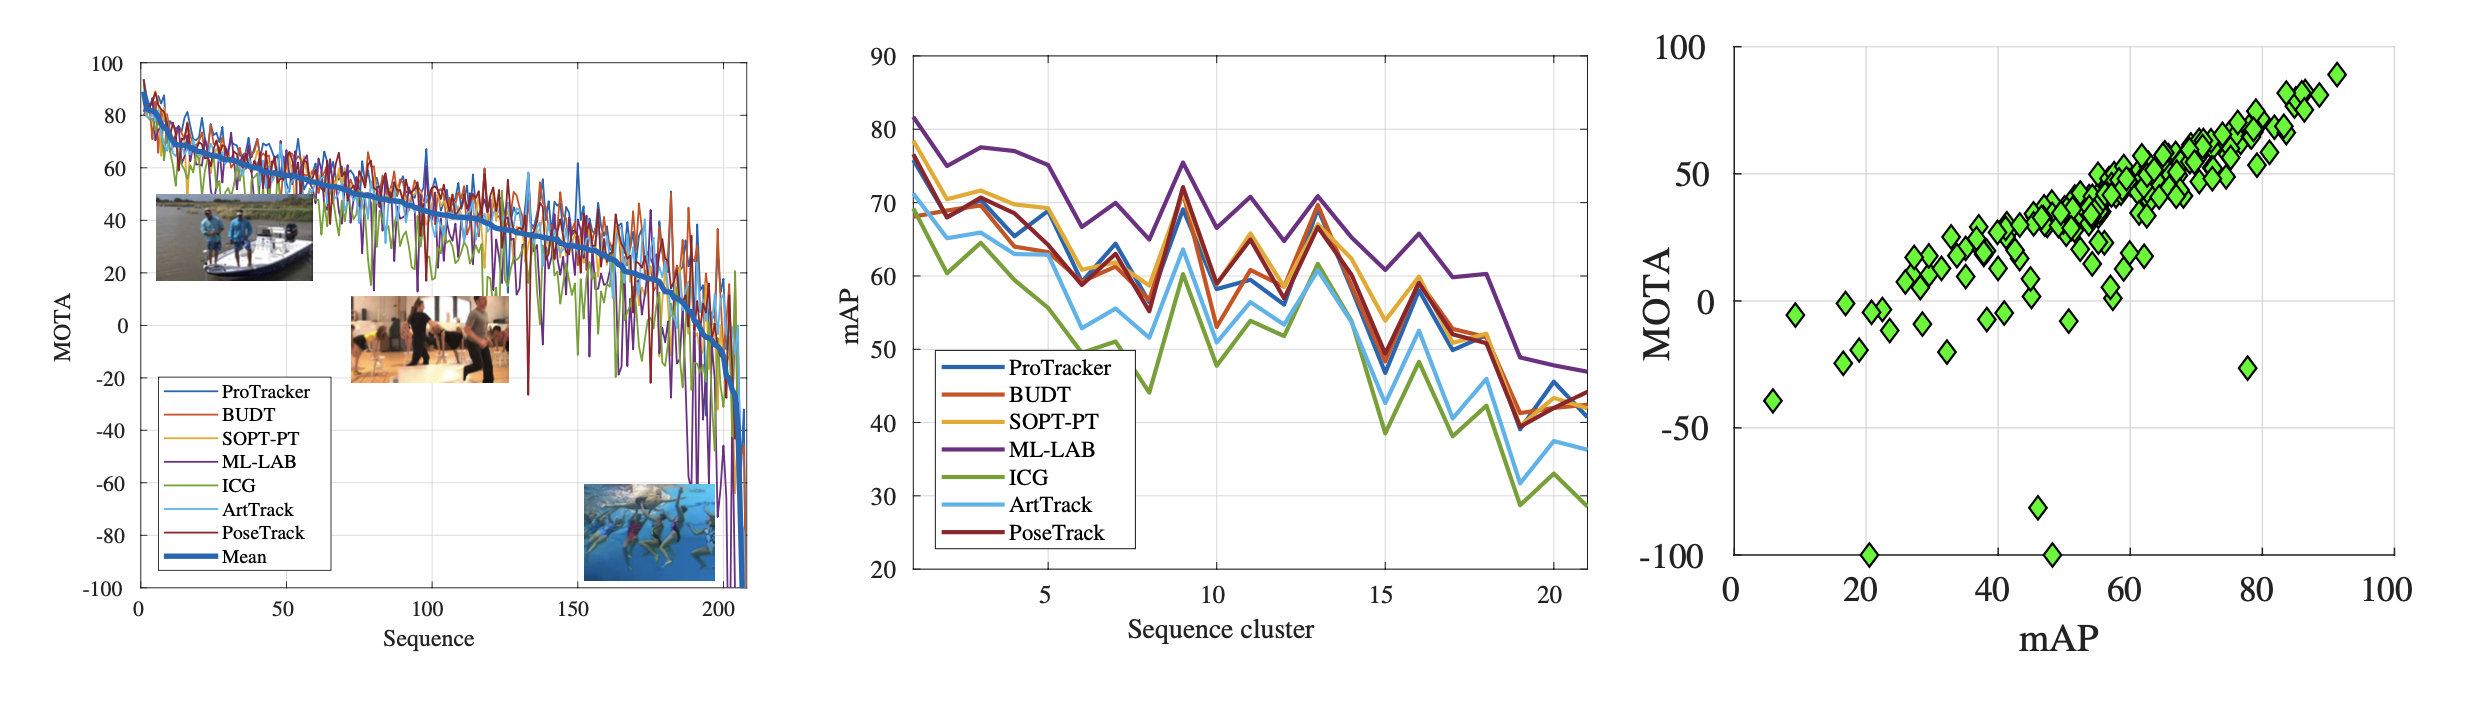
\includegraphics[width=\textwidth]{figs/metrics.png} 
    \caption{Sequences sorted by average MOTA (left). Pose estimation results
    sorted by articulation complexity of the sequence (middle). Correlation
    between mAP and MOTA for each sequence (right). Reproduced from
    \cite{andriluka2018posetrack}.}
    \label{fig:mota_map}
\end{figure}

\subsection{Visual Representation} The second method for representing pose
tracking results is through visualizations \ref{fig:visualizations}. This
approach involves drawing the detected keypoints on each person and connecting
them with lines, creating a stickman-like skeleton. This visual representation
not only shows the positions of the keypoints but also illustrates the
relationships between them, making it easier to interpret the pose of each
person in a scene.

By connecting the keypoints with lines, one can clearly see the structure of the
pose, including the positions of limbs and joints. This visual representation is
particularly useful for quickly assessing the accuracy and quality of the pose
tracking results, as it provides an intuitive way to verify whether the
keypoints have been correctly identified and connected.

\begin{figure}[ht!]
    \centering
    \begin{subfigure}[b]{0.3\textwidth}
        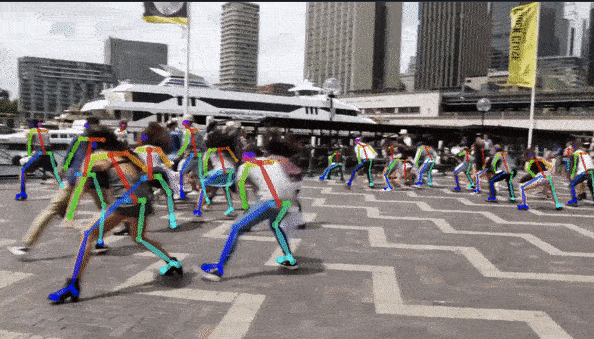
\includegraphics[width=\textwidth]{figs/openpose.png} 
        \caption{From \cite{cao2017realtime}}
        \label{fig:openpose}
    \end{subfigure}
    \hfill
    \begin{subfigure}[b]{0.3\textwidth}
        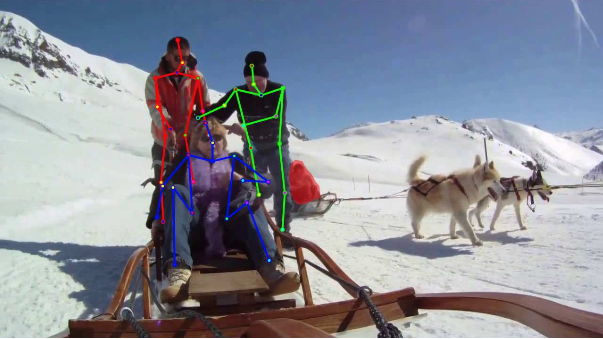
\includegraphics[width=\textwidth]{figs/posetrack.png}
        \caption{From \cite{andriluka2018posetrack}}
        \label{fig:posetrack}
    \end{subfigure}
    \hfill
    \begin{subfigure}[b]{0.3\textwidth}
        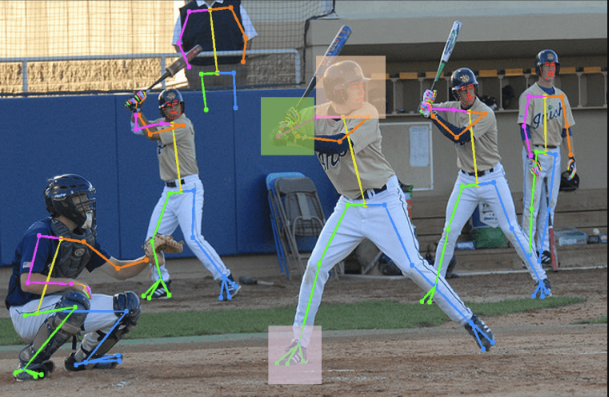
\includegraphics[width=\textwidth]{figs/coco-wholebody.png}
        \caption{From \cite{jin2020whole}}
        \label{fig:coco-wholebody}
    \end{subfigure}
    \begin{subfigure}[b]{0.3\textwidth}
        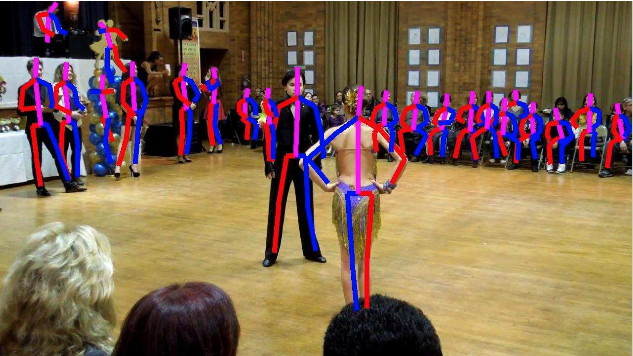
\includegraphics[width=\textwidth]{figs/fang-rmpe.png}
        \caption{From \cite{fang2017rmpe}}
        \label{fig:fang-rmpe}
    \end{subfigure}
    \begin{subfigure}[b]{0.3\textwidth}
        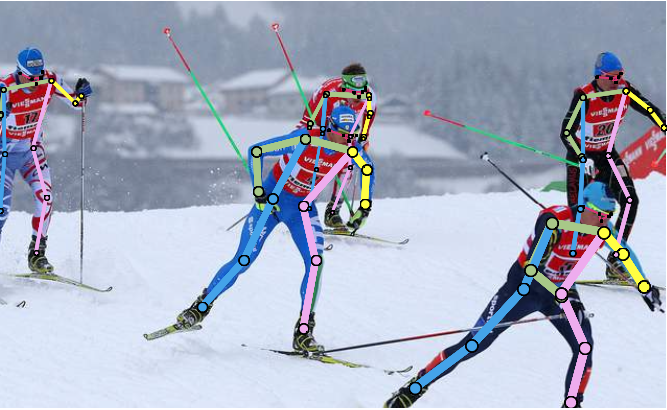
\includegraphics[width=\textwidth]{figs/sundeep.png}
        \caption{From \cite{sun2019deep}}
        \label{fig:sundeep}
    \end{subfigure}
    \begin{subfigure}[b]{0.3\textwidth}
        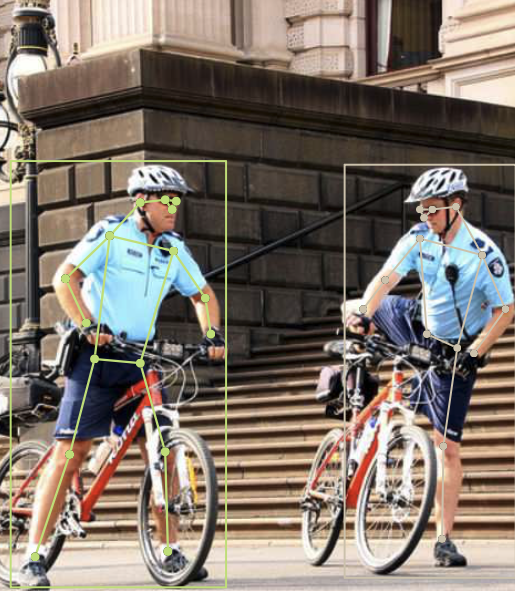
\includegraphics[width=\textwidth]{figs/papandreou.png}
        \caption{From \cite{Papandreou_2017_CVPR}}
        \label{fig:papandreou}
    \end{subfigure}
    \begin{subfigure}[b]{0.3\textwidth}
        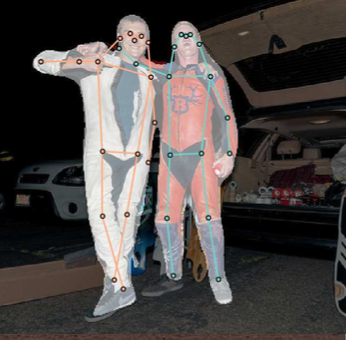
\includegraphics[width=\textwidth]{figs/kokabas.png}
        \caption{From \cite{Kocabas_2018_ECCV}}
        \label{fig:kocabas}
    \end{subfigure}
    \begin{subfigure}[b]{0.3\textwidth}
        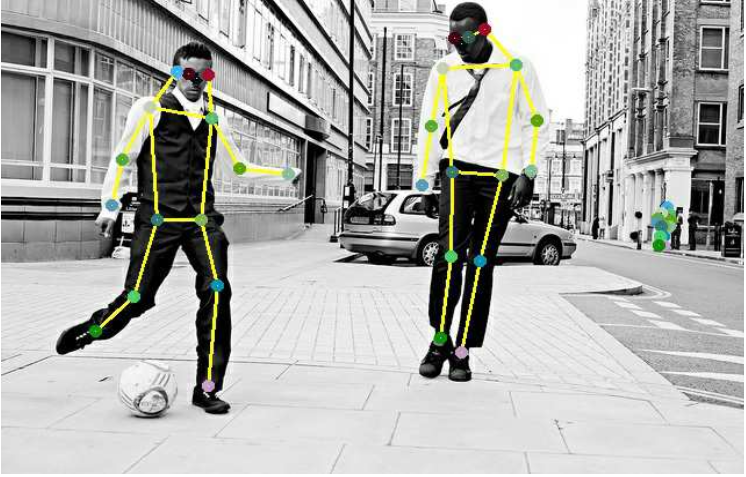
\includegraphics[width=\textwidth]{figs/chen.png}
        \caption{From \cite{chen2018cascaded}}
        \label{fig:chen}
    \end{subfigure}
    \begin{subfigure}[b]{0.3\textwidth}
        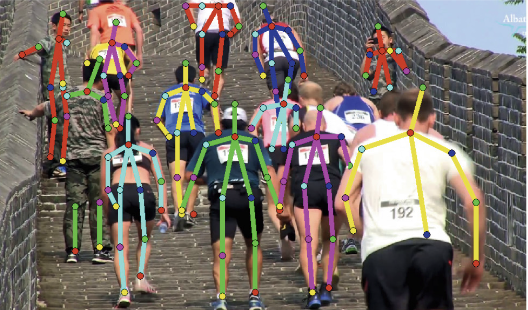
\includegraphics[width=\textwidth]{figs/deeper.png}
        \caption{From \cite{insafutdinov2016deepercut}}
        \label{fig:deeper}
    \end{subfigure}
    \caption{Visual representation from a number of different multi person pose estimation papers}
    \label{fig:visualizations}
\end{figure}

Both metric-based and visual representations are essential for thoroughly
evaluating and demonstrating the effectiveness of multi-person pose tracking
systems. While metrics provide a quantitative assessment, visualizations offer
an immediate, interpretable view of the results, making them complementary tools
in pose tracking analysis.

\section{Significance}

By combining monocular depth cues with a graph-based attention model, this
research offers a new route to multi-person pose tracking that is both accurate
and computationally lean.  Augmenting each joint with a depth value lifts the
skeleton into 2.5-D space, giving the Graph Attention Network (GAT) geometric
context that pure 2-D coordinates lack.  The resulting graph encodes only a
small set of informative features, lowering memory usage and shortening
training time while enabling real-time inference on modest hardware.  

Because the framework accepts keypoints from any detector that follows a known
joint schema, it can track advances in front-end pose estimation without
architectural changes. This detector-agnostic design, coupled with the compact
feature space, creates a scalable solution for applications ranging from crowd
analytics and sports performance to augmented reality and human-robot
interaction.

\bibliography{refs}{}
\bibliographystyle{IEEEtran}

\end{document}
